%=============================================================


\begin{figure}[!htbp]
\centering
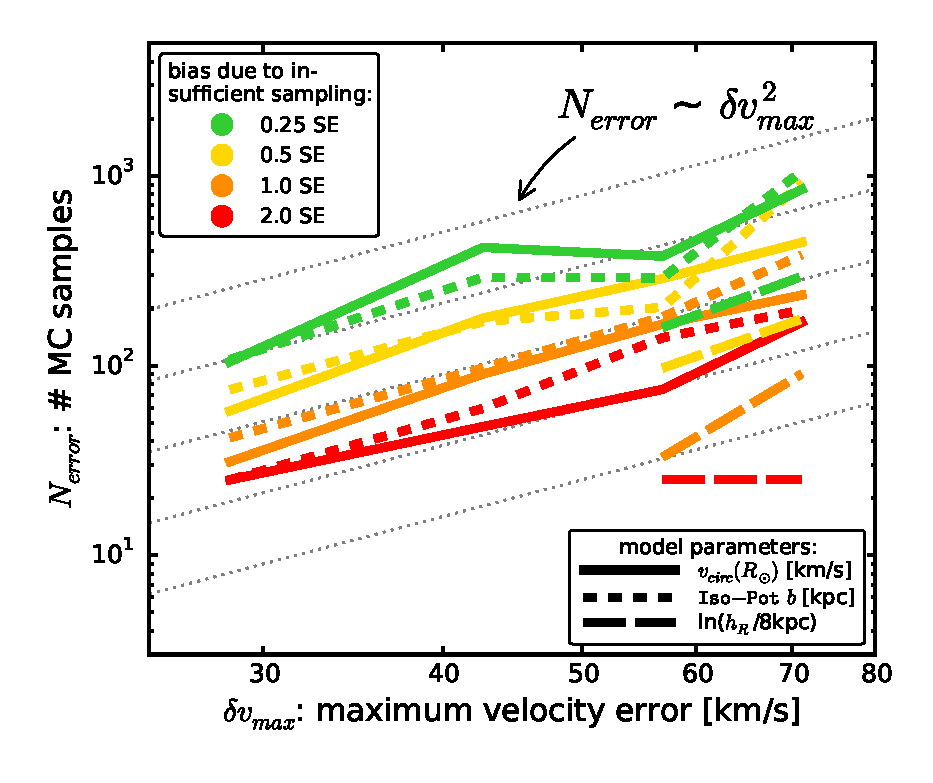
\includegraphics[width=\columnwidth]{figs/isoSphFlexErrConv_MC_vs_error_2.eps}
\caption{Number of Monte Carlo (MC) samples $N_\text{error}$ needed for the numerical convolution of the model probability with the measurement uncertainties in Equation \ref{eq:errorconv}, given the maximum velocity uncertainty $\delta v_\text{max}$ within the stellar sample. Insufficient sampling introduces systematic biases in the parameter recovery as indicated in the legend. The relation found here, $N_\text{error} \propto \delta v_\text{max}^2$, was distilled from a set of analyses of mock data sets with different proper motion uncertainties $\delta \mu \in [2,5]~\text{mas yr}^{-1}$ in the absence of distance uncertainties (see Test \ref{test:isoSphFlexErrConv_MC_vs_error} in Table \ref{tbl:tests}). The proper motion uncertainty $\delta \mu$ translates to heteroscedastic \Wilma{[TO DO: make sure that this word is written correctly everywhere.]} velocity uncertainties according to $\delta v [\text{km s}^{-1}] \equiv 4.74047 \cdot r[\text{kpc}] \cdot \delta \mu [\text{mas yr}^{-1}]$, with $r$ being the distance of the star from the Sun. Stars with larger $\delta v$ require more $N_\text{error}$ for the integral over its measurement uncertainties to converge. We therefore show how the $N_\text{error}$ needed for the potential \pdf{} of the whole data set to be converged, depends on the largest velocity error $\delta v_\text{max} \equiv \delta v(r_\text{max})$ within the data set. We used $N_\text{error} = 800$ and  $1200$ for $\delta \mu \leq 3 \text{mas yr}^{-1}$ and $\delta \mu > 3 \text{mas yr}^{-1}$, respectively, as the reference for the converged convolution integral (see also left panels in Figure \ref{fig:isoSphFlexErrConv_bias_vs_SE}). This figure was generated from mock data sets with $N_{*}=10,000$. We found that for $N_{*}=5,000$ the required $N_{error}$ remains similar for $b$, but gets smaller for $v_\text{circ}(R_\odot)$. Overall we expect that we need less accuracy and therefore smaller $N_\text{error}$ for smaller $N_{*}$. \Wilma{[TO DO: some of the 25 MC sample analyses have to be re-done.] [TO DO: Use $N_*$ everywhere where applicable, no $N_\text{sample}$] [TO DO: Introduce $N_*$ somewhere.]}}
\label{fig:isoSphFlexErrConv_MC_vs_error}
\end{figure}

%=============================================================

%====================================================================

%FIGURE: Triangle plot, shape of likelihood, multi-variate Gaussian

\begin{figure*}[!htbp]
\centering
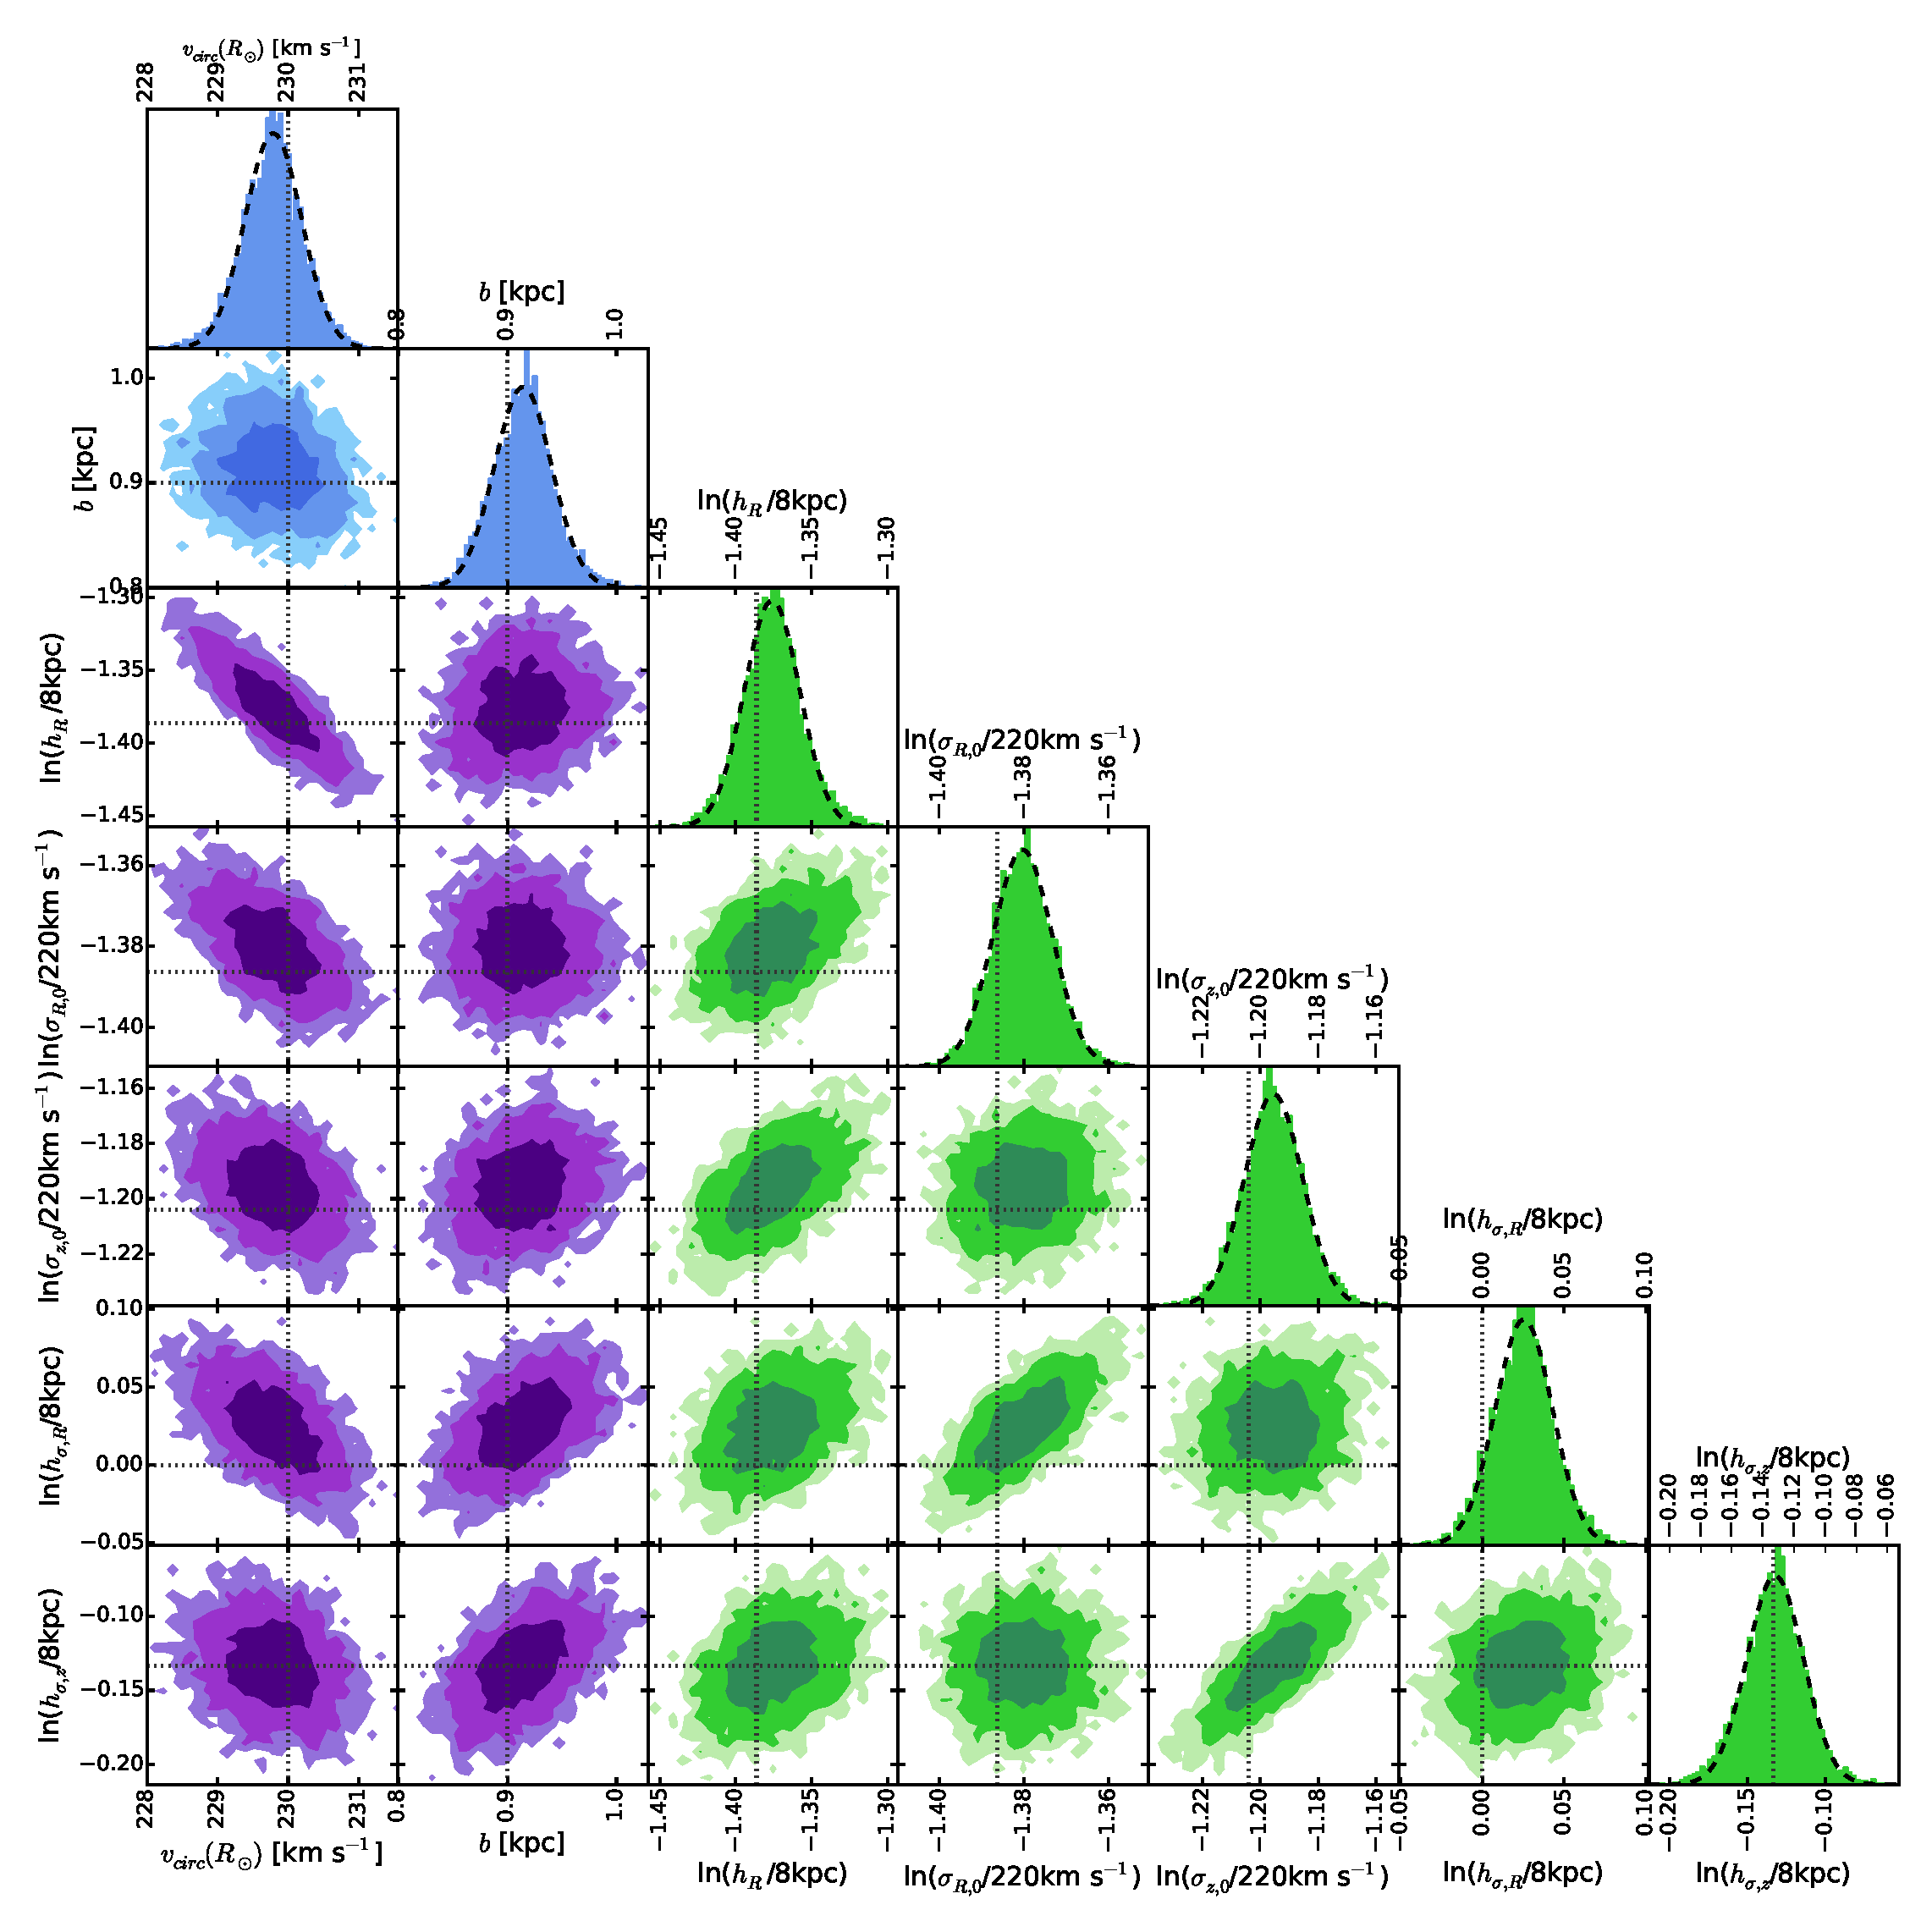
\includegraphics[width=0.7\textwidth]{figs/isoSphFlex_short_hot_2kpc_triangle_MCMC.eps}
\caption{The \pdf{} (proportional to the likelihood in Equation \ref{eq:prob}) in the parameter space $\pmodel{} = \{p_\Phi,p_\text{DF}\}$ for one example mock data set created according to Test \ref{test:isoSphFlex} in Table \ref{tbl:tests}. Blue indicates the \pdf{} for the potential parameters, green the qDF parameters. The true parameters are marked by dotted lines. The dark, medium and bright contours in the 2D distributions represent 1, 2 and 3 sigma confidence regions \HW{[TO DO: HW: "likelihood vs. pdf - This is where this matters: is this a confidence on the data or on the parameters?" Don't understand, what he means...]}, respectively. The parameters are weakly to moderately covariant, but their level of covariance depends on the actual choice of the mock data's \pmodel{}. The \pdf{} here was sampled using MCMC. The dashed lines in the 1D distributions are Gaussian fits to the histogram of MCMC samples. This demonstrates very well that for such a large number of stars, the \pdf{} approaches the shape of a multi-variate Gaussian, as expected for an maximum likelihood estimator.}
\label{fig:isoSphFlex_triangleplot}
\end{figure*}

%====================================================================


\subsection{Data Likelihood} \label{sec:likelihood}


As data we consider here the positions and velocities of a population of stars within a given survey selection function $\text{SF}(\vect{x})$,
\begin{eqnarray*}
D  =\{ \vect{x}_i,\vect{v}_i \mid && \text{(star $i$ in given stellar population)}\nonumber\\
&\wedge& (\text{SF}(\vect{x_i}) > 0) \}.
\end{eqnarray*}

We fit a model potential and DF (here: the qDF) which are specified by a number of fixed and free parameters,
\begin{eqnarray*}
\pmodel \equiv \{ p_\text{DF} , p_\Phi \}.
\end{eqnarray*}
The orbit of the $i$-th star in a potential with $p_\Phi$ is labeled by the actions $\vect{J}_i := \vect{J}[\vect{x}_i,\vect{v}_i\mid p_{\Phi}]$ and the DF evaluated for the $i$-th star is then $\text{DF}(\vect{J}_i \mid \pmodel) := \text{DF}(\vect{J}[\vect{x}_i,\vect{v}_i\mid p_{\Phi}] \mid p_\text{DF})$.\\

The likelihood of the data given the model is, following BR13,
\begin{eqnarray}
&&\mathscr{L}(D \mid \pmodel) \nonumber\\
&&\equiv \prod_i^{N_*} p(\vect{x}_i,\vect{v}_i \mid \pmodel) \nonumber\\
&&= \prod_i^{N_*} \frac{\text{DF}(\vect{J}_i \mid \pmodel) \cdot \text{SF}(\vect{x}_i)}{\int \Diff 3 x \Diff 3 v \  \text{DF}(\vect{J} \mid \pmodel) \cdot \text{SF}(\vect{x})}\nonumber\\
&&\propto \prod_i^{N_*} \frac{\text{DF}(\vect{J}_i \mid \pmodel)}{\int \Diff 3 x \  \rho_\text{DF}(R,|z| \mid \pmodel) \cdot \text{SF}(\vect{x})}, \label{eq:prob}
%\label{eq:likelihood}
\end{eqnarray}
where $N_*$ is the number of stars in $D$, and in the last step we used Equation \ref{eq:tracerdensity}. $\prod_i\text{SF}(\vect{x}_i)$ is independent of \pmodel{}, so we treat it as unimportant proportionality factor. We find the best fitting \pmodel{} by maximizing the posterior probability distribution $\pdf{}(\pmodel \mid D)$, which is, according to Bayes' theorem, proportional to the likelihood $\mathscr{L}(D\mid \pmodel)$ times a prior $p(\pmodel)$. We assume flat priors in both $p_\Phi$ and
\begin{eqnarray}
p_\text{DF} := \{ \ln h_R, \ln \sigma_{R,0}, \ln \sigma_{z,0}, \ln h_{\sigma,R}, \ln h_{\sigma,z} \} \label{eq:p_DF}
\end{eqnarray}
(see Section \ref{sec:qDF}) throughout this work. Then \pdf{} and likelihood can be used interchangeably.\\

The normalisation in Equation \ref{eq:prob} is a measure for the total number of tracers inside the survey volume,
\begin{equation}
M_\text{tot} \equiv \int \Diff 3 x \  \rho_\text{DF}(R,|z| \mid \pmodel) \cdot \text{SF}(\vect{x}).\label{eq:normalisation}
\end{equation}
In the case of an axisymmetric galaxy model and $\text{SF}(\vect{x})=1$ within the observation volume (as in most tests in this work), the normalisation is essentially a two-dimensional integral in the $R$-$z$ plane over $\rho_{DF}$. We evaluate the integrals using Gauss-Legendre quadratures of order 40. The integral over the azimuthal direction can be solved analytically. 
\\It turns out that a sufficiently accurate evaluation of the likelihood is computationally expensive, even for only one set of model parameters. This expense is dominated by the number of action calculations required, which in turn depends on the number of stars in the sample ($N_*$ action calculations) and the numerical accuracy of the tracer density grid in Equation \ref{eq:tracerdensity} needed for the likelihood normalization in Equation \ref{eq:normalisation} ($N_x^2 \times N_v^3$ action calculations). The accuracy has to be chosen high enough, such that the resulting numerical error 
\begin{equation}
\delta_{M_\text{tot}} \equiv \frac{M_\text{tot,approx}(N_x,N_v,n_\sigma) -  M_\text{tot} }{M_\text{tot}}\label{eq:relerrlikelihood}
\end{equation}
does not dominate the numerically calculated log-likelihood, i.e.,
\begin{eqnarray}
& &\log \mathscr{L}_\text{approx}(D \mid \pmodel) \nonumber\\
&& = \sum_i^{N_*} \log \text{DF}(\vect{J_i} \mid \pmodel) - N_* \log(M_\text{tot})\nonumber\\
&& - N_* \log (1 + \delta_{M_\text{tot}}),\label{eq:loglikelihood_relerr}
\end{eqnarray}
with
\begin{eqnarray}
N_* \log (1 + \delta_{M_{tot}}) \leq 1.\nonumber
\end{eqnarray}
Otherwise numerical inaccuracies could lead to systematic biases in the potential and DF recovery. For data sets as large as $N_* = 20,000$ stars, which in the age of Gaia could very well be the case \HW{[TO DO: Really???]}, one needs a numerical accuracy of 0.005\% in the normalisation. Figure \ref{fig:norm_accuracy} demonstrates that the numerical accuracy we use in the analysis, $N_x=16$, $N_v=24$ and $n_\sigma=5$, does satisfy this requirement. This is slightly higher than in BR13, where $N_* \sim 100$ \Wilma{[TO DO: CHECK]}.\\


%====================================================================

Measurement uncertainties of the data have to be incorporated in the likelihood. We assume Gaussian uncertainties in the observable space $\vect{y} \equiv (\tilde{\vect{x}},\tilde{\vect{v}})=(\text{RA},\text{Dec},(m-M),\mu_\text{RA} \cdot \cos \text{Dec},\mu_\text{Dec},v_\text{los})$, i.e. the $i$-th star's observed $\vect{y}_i$ are drawn from the normal distribution $N[{\vect{y}'}_i,\delta \vect{y}_i]$, with ${\vect{y}_i}'$ being the star's true phase-space position and $\delta \vect{y}_i$ its uncertainty . Stars follow the distribution function (DF$(\vect{y}') \equiv$ DF$(\vect{J}[\vect{y}' \mid p_\Phi] \mid p_\text{DF})$ for short), convolved with the measurement uncertainties $N[0,\delta \vect{y}]$ \Wilma{[TO DO: CHECK AGAIN]}. The selection function SF$(\vect{y})$ acts on the space of (error affected) observables. Then the probability of one star becomes
\begin{eqnarray*}
&&\tilde{p}(\vect{y}_i \mid p_\Phi,p_\text{DF},\delta \vect{y}_i)\\
& \equiv& \frac{\text{SF}(\vect{y}_i) \cdot \int \Diff{6} y' \  \text{DF}(\vect{y}') \cdot N[\vect{y}_i,\delta \vect{y}_i]}{\int \Diff{6}y'  \  \text{DF}(\vect{y}')  \cdot  \int \Diff{6} y \  \text{SF}(\vect{y})  \cdot N[\vect{y}',\delta \vect{y}_i]}.
\end{eqnarray*}
In the case of uncertainties in distance or (RA,Dec), the evaluation of this is computational expensive - especially if the stars have heteroscedastic $\delta \vect{y}_i$. In practice we apply the following approximation,
\begin{eqnarray}
&&\tilde{p}(\vect{y}_i \mid p_\Phi,p_\text{DF},\delta \vect{y}_i) \nonumber\\
&&\approx \frac{ \text{SF}(\vect{x}_i)}{M_\text{tot}} \cdot \frac{1}{N_\text{error}} \sum_n^{N_\text{error}}  \text{DF}(\vect{x}_i,\vect{v}[\vect{y}'_{i,n}]) \label{eq:errorconv}
\end{eqnarray}
with
\begin{eqnarray}
\vect{y}'_{i,n} \sim N[\vect{y}_i,\delta \vect{y}_i]\nonumber
\end{eqnarray}
We calculate the convolution using Monte Carlo (MC) integration with $N_\text{error}$ samples. The above approximation assumes that the star's \emph{position} $\vect{x}_i$ is perfectly measured. As the selection function is also velocity independent, this simplifies the normalisation drastically to Equation \ref{eq:normalisation}. Measurement uncertainties in $\mathrm{RA}$ and $\mathrm{Dec}$ are often negligible anyway. The uncertainties in the Galactocentric \emph{velocities} $\vect{v}_i = (v_{R,i},v_{T,i},v_{z,i})$ depend besides on $\delta \vect{\mu}$ and $\delta v_\text{los}$ also on the distance and its uncertainty, which we do \emph{not} neglect when drawing MC samples $\vect{y}'_{i,n}$ from the full uncertainty distribution $N[\vect{y}_i,\delta \vect{y}_i]$. Figure \ref{fig:isoSphFlexErrConv_MC_vs_error} demonstrates that in the absence of position uncertainties the $N_\text{error}$ needed for the convolution integral to converge depends as
\begin{equation*}
N_\text{error} \propto \delta v^2
\end{equation*}
on the uncertainties in the (1D) velocities. We found that the required $N_\text{error}$ to reach a given accuracy does not depend strongly on the number of stars in the sample. But in general we expect that we need higher accuracy and therefore more $N_\text{error}$ for larger data sets.
\\A similar but only one-dimensional treatment of measurement uncertainties in $v_z$ was already applied by BR13.

